\documentclass{article}

% Template from:  https://samrobbins.uk/blog/my-latex-boilerplate
% Plotting from:  https://latex-tutorial.com/tutorials/pgfplots/
%
% Generate output in a terminal using:
% pdflatex prandtlAirfoils.tex
%
% Doen eers hierdie opdragte:
% Bibliografie vertaling
%bibtex prandtlAirfoils
% Die nomenklatuurvertaling
%makeindex prandtlAirfoils.glo -s nomencl.ist -o prandtlAirfoils.gls


\usepackage{graphicx}
\usepackage{float}
\usepackage{natbib}
\usepackage{tikz}
\usepackage{pgfplots}
\usepackage{siunitx}


\pgfplotsset{compat=newest} % Allows to place the legend below plot
\usepgfplotslibrary{units} % Allows to enter the units nicely

\sisetup{
  round-mode          = places,
  round-precision     = 2,
}

% Include all the macros to plot the polars
% Contains all the macros or newcommands

\newcommand{\avector}[2]{(#1_1,#1_2,\ldots,#1_{#2})}


% Expects a CSV file that is similar to XFOIL output, then plot the following
% CL versus alpha

\newcommand{\oomparepolar}[3]{
\begin{figure}[H]
  \begin{center}
    \begin{tikzpicture}
      \begin{axis}[
          width=\linewidth, % Scale the plot to \linewidth
          grid=major, % Display a grid
          grid style={dashed,gray!30}, % Set the style
          xlabel=$\alpha$, % Set the labels
          ylabel=$C_L$,
          x unit=\si{\degree}, % Set the respective units
          y unit=\si{},
          legend style={at={(0.5,-0.2)},anchor=north}, % Put the legend below the plot
          x tick label style={rotate=90,anchor=east} % Display labels sideways
        ]
        \addplot 
        % add a plot from table; you select the columns by using the actual name in
        % the .csv file (on top)
        table[x=alpha,y=CL,col sep=comma] {#1}; 
		\addplot
		table[x=alpha,y=CL,col sep=comma] {#2}; 
        \legend{#1, #2}
      \end{axis}
    \end{tikzpicture}
    \caption{#3}
  \end{center}
\end{figure}
}

% Plot the coefficient versus angle of attack
% Usage:
% \makecoeffplot{../HQ34/hq34Polar.csv}{Aerodynamic data of HQ34.}{CL}
% Plots the *.csv file with the title in the second variable, the CL parameter


\newcommand{\makecoeffplot}[3]{
\begin{figure}[H]
  \begin{center}
    \begin{tikzpicture}
      \begin{axis}[
          width=0.5\linewidth, % Scale the plot to \linewidth
          grid=major, % Display a grid
          grid style={dashed,gray!30}, % Set the style
          xlabel=$\alpha$, % Set the labels
          ylabel=#3,
          x unit=\si{\degree}, % Set the respective units
          y unit=\si{},
          legend style={at={(0.5,-0.2)},anchor=north}, % Put the legend below the plot
          x tick label style={rotate=90,anchor=east} % Display labels sideways
        ]
        \addplot 
        % add a plot from table; you select the columns by using the actual name in
        % the .csv file (on top)
        table[x=alpha,y=#3,col sep=comma] {#1}; 
      \end{axis}
    \end{tikzpicture}
    \caption{#2}
  \end{center}
\end{figure}
}




% Expects a CSV file with x/c in first column, CSV, then plot the following
% Cp versus x/c

\newcommand{\oompareCP}[3]{
\begin{figure}[H]
  \begin{center}
    \begin{tikzpicture}
      \begin{axis}[
          width=\linewidth, % Scale the plot to \linewidth
          grid=major, % Display a grid
          grid style={dashed,gray!30}, % Set the style
          xlabel=$\frac{x}{c}$, % Set the labels
          ylabel=$C_p$,
          x unit=\si{}, % Set the respective units
          y unit=\si{},
          legend style={at={(0.5,-0.2)},anchor=north}, % Put the legend below the plot
          x tick label style={rotate=90,anchor=east} % Display labels sideways
        ]
        \addplot 
        % add a plot from table; you select the columns by using the actual name in
        % the .csv file (on top)
        table[x=xc,y=Cp,col sep=comma] {#1}; 
		\addplot
		table[x=xc,y=Cp,col sep=comma] {#2}; 
        \legend{#1, #2}
      \end{axis}
    \end{tikzpicture}
    \caption{#3}
  \end{center}
\end{figure}
}

\newcommand{\plotpolar}[2]{
\begin{figure}[H]
  \begin{center}
    \begin{tikzpicture}
      \begin{axis}[
          width=\linewidth, % Scale the plot to \linewidth
          grid=major, % Display a grid
          grid style={dashed,gray!30}, % Set the style
          xlabel=$C_D$, % Set the labels
          ylabel=$C_L$,
          x unit=\si{}, % Set the respective units
          y unit=\si{},
          legend style={at={(0.5,-0.2)},anchor=north}, % Put the legend below the plot
          x tick label style={rotate=90,anchor=east} % Display labels sideways
        ]
        \addplot 
        % add a plot from table; you select the columns by using the actual name in
        % the .csv file (on top)
        table[x=CD,y=CL,col sep=comma] {#1}; 
      \end{axis}
    \end{tikzpicture}
    \caption{#2}
  \end{center}
\end{figure}
}




\title{Airfoil analysis on the Prandtl D and the SB-13 aircraft}
\author{Ni\"el Agenbag}
\date{2024-01-08}


\begin{document}

\maketitle

Report data for the aerodynamic analysis for the Prandtl wing airfoils.

Put report data here:

\section{Introduction}


To do:
Analyse HQ36 and document with XFOIL
Analyse Prandtl root and tip and document with XFOIL
Write LaTeX macro to plot drag polar.
CFD all profiles.  Use OpenFoam
Insert benchmark results with NACA 23012
Also plot over windtunnel results of the HQ profiles and the NACA23012
Compare windtunnel, CFD and XFOIL.  Check how close predictions are.

$\mathbf u=\avector{u}{7}$


\section{NACA 23012}

plot airfoil
plot cl, cd vs alpha

\section{HQ34}

Digitized the HQ34 from .


\begin{figure}[H]
	\begin{center}
		\begin{tikzpicture}
	 		\draw[scale=10] plot file{../HQ34/mdesOnly/HQ34smoothPic.dat} -- cycle;
		\end{tikzpicture}
	\end{center}
	\caption{Vlerkprofiel van die HQ34.}
	\label{Fig: Vlerkprofiel HQ34}
\end{figure}


Then smoothed the profile using the MDES command FILT.
Then ran a polar to obtain the following result:
Viscous analysis with Reynolds number = 100000.

\begin{figure}[H]
\centering
\includegraphics[width=\textwidth]{../HQ34/mdesOnly/hq34Polar.pdf}
\caption{HQ34 polar from digitized profile.}
\end{figure}



% Plot the polar plots:
\makecoeffplot{../HQ34/mdesOnly/hq34Polar.csv}{Aerodynamic data of HQ34.}{CL}
\makecoeffplot{../HQ34/mdesOnly/hq34Polar.csv}{Aerodynamic data of HQ34.}{CD}
\makecoeffplot{../HQ34/mdesOnly/hq34Polar.csv}{Aerodynamic data of HQ34.}{CM}
\makecoeffplot{../HQ34/mdesOnly/hq34Polar.csv}{Aerodynamic data of HQ34.}{CDp}

The Akaflieg Braunschweig SB-13 airfoil profile properties are obtained from \cite{SB13Aerodynamics}.

\oomparepolar{../HQ34/mdesOnly/hq34Polar.csv}{../HQ34/hq34Polartest.csv}{Compare analysis to test}

These results are unacceptable.  It looks like the flow is tripped by the irregular geometry.  The MDES FILT smoothing seems to be insufficient on its own.  Got better results with spline interpolation of digitized points.
Run the cscvn spline fit function again on the new digitized points.  Compare the old digitized points results with the new interpolated results.


Here is the old Cp comparison:

\oompareCP{../HQ34/HQ34XFOILAlpha45Re1e6.csv}{../HQ34/HQ34windtonnelAlpha45Re1e6.csv}{Compare XFOIL analysis to windtunnel Cp}


Here is a drag polar with the bad data:

\plotpolar{../HQ34/mdesOnly/hq34Polar.csv}{Polar of the XFOIL data}

When the following zoomed plot is investigated the noise of the digitized profile is visible.

\begin{figure}[H]
\centering
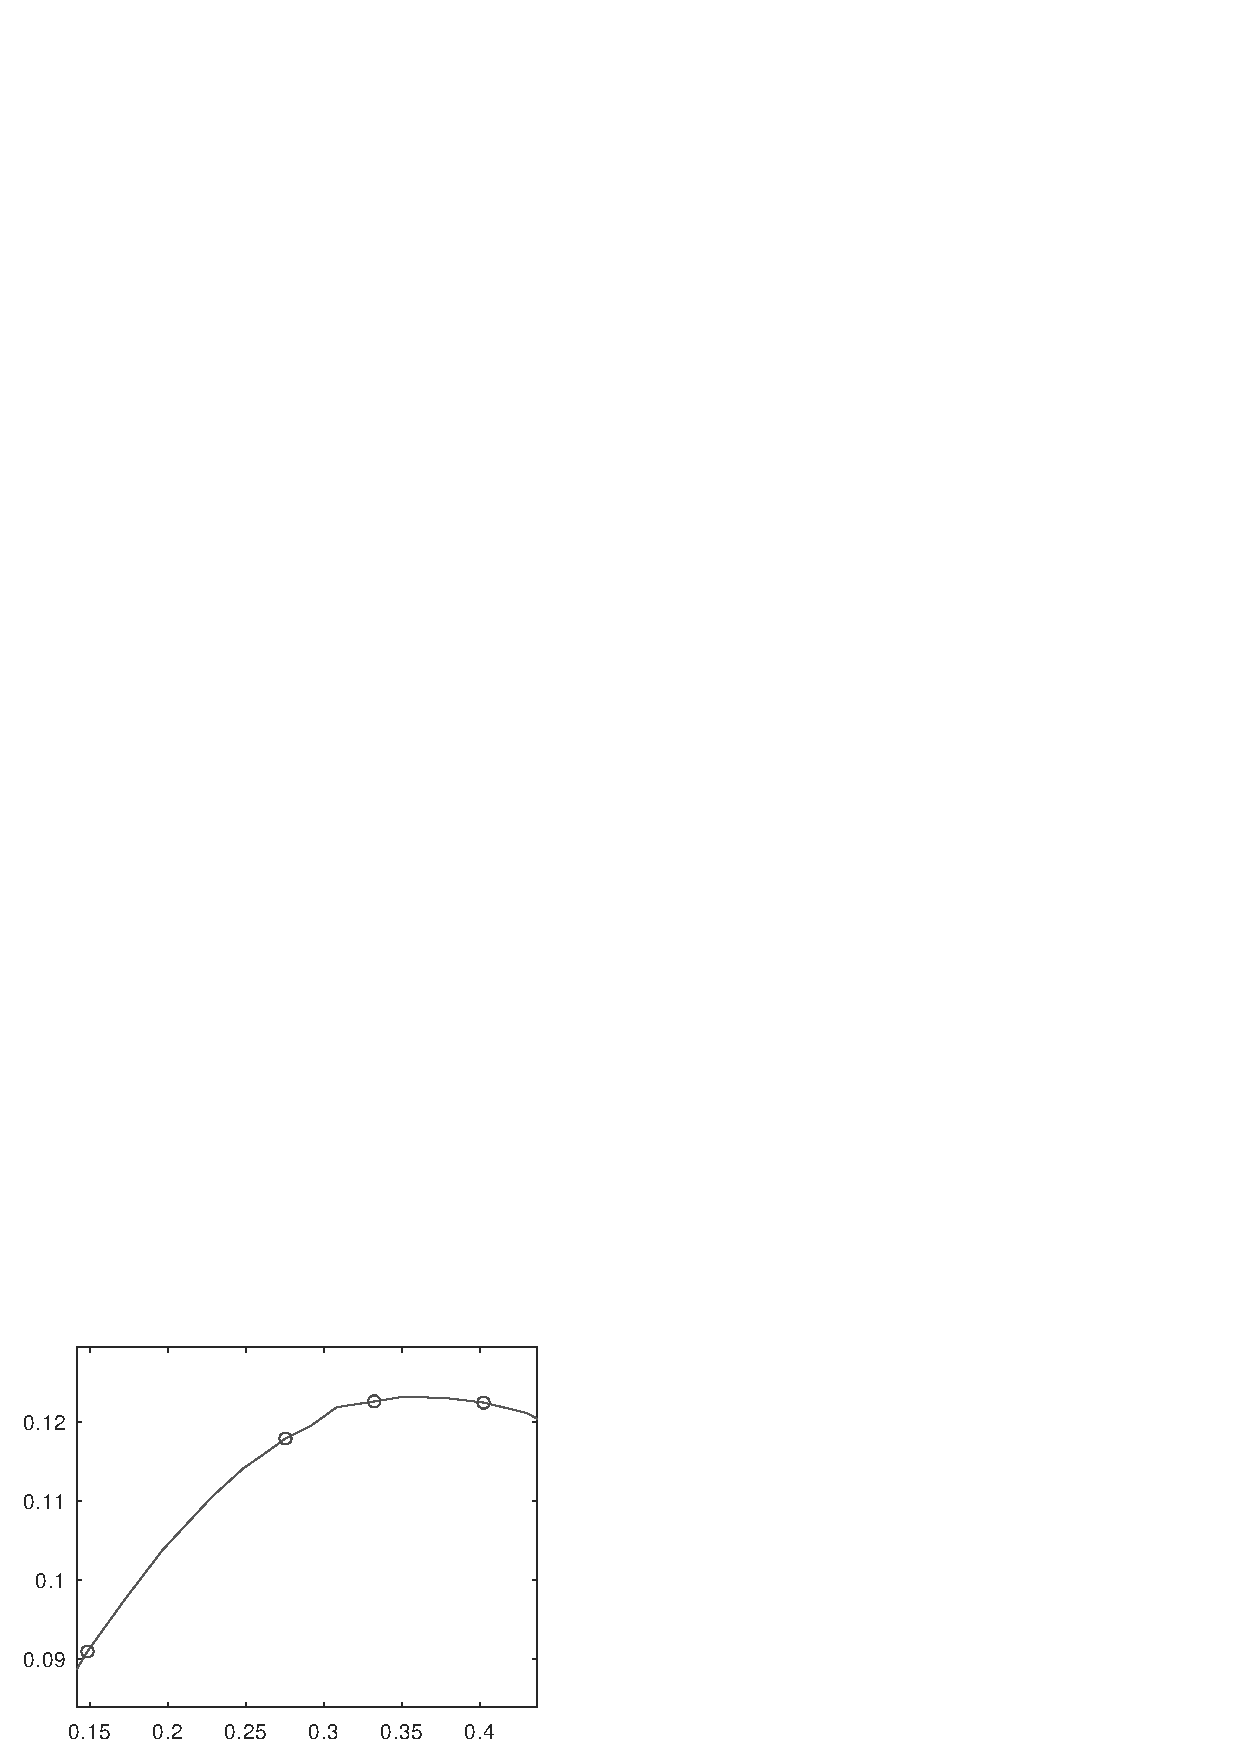
\includegraphics[width=\textwidth]{../HQ34/cscvnMdes/HQ34wysGeraas.pdf}
\caption{Potential issue with HQ34 digitized profile that causes mathematical noise.}
\end{figure}

\section{HQ36}


\section{Prandtl D root}

\subsection{XFOIL analysis}

\subsection{CFD}

\section{Prandtl D tip}



\bibliography{prandtlAirfoils}
\bibliographystyle{cheming}

\end{document}
